% !TEX root = ../thesis-example.tex
%
\chapter{Forecasting discount curves with Kernel Regularized Least Squares}
\label{sec:discount_curve_krls}

%\cleanchapterquote{Users do not care about what is inside the box, as long as the box does what they need done.}{Jef Raskin}{about Human Computer Interfaces}

\section{Introduction}

In this chapter, we apply Kernel Regularized Least Squares (KRLS) learning methods to Yield Curve forecasting. By 'Yield Curve', we actually mean a discount curves. That is, we consider that the curves used in theexamples do not include counterparty credit risk, and we focus on the forecasting problem. Two types of formulations of the forecasting problem are tested. One relying on the popular Dynamic Nelson-Siegel (DNS) framework from \cite{diebold2006forecasting}, and another one, in which we apply the KRLS directly to the Yield Curve observation dates and time to maturities, to model the spot rates.

\medskip

In the DNS framework \cite{diebold2006forecasting}, each cross-section of yields observed over time is fitted by using the Nelson-Siegel \cite{nelson1987parsimonious} model. This cross-section fitting produces three time series of parameters (more details in the next section) representing the evolution of the level, slope, and curvature of the Yield Curve. The KRLS model  is applied to forecasting  the time series of parameters, using a technique which is similar to the one described in \cite{exterkate2016nonlinear}. And to finish, the forecast obtained for the trivariate time series are plugged into the Nelson-Siegel model, to deduce forecast for the cross-sections of yields.

\medskip

The second approach is a machine learning/data-driven one, in which we put no  specific constraint on the model to reproduce the specific Yield Curve stylized facts. The regularization parameters inherent to the KRLS model will act as implicit constraints, that cause the model to converge as close as possible to reproducing these stylized facts. In this latter approach, we are mostly interested in the model with the {\it best} out-of-sample error. As a consequence, the technique as is, is probably less adapted than the former framework based on DNS (in its arbitrage-free version) to no-arbitrage pricing (if no-arbitrage pricing is required).

\medskip

To introduce KRLS, we start by describing the ridge regression \cite{hoerl1970ridge} and the {\it kernel trick} applied to ridge regression. Then, we make a link between this kernel ridge regression and KRLS. In a ridge regression setting, we want to explain an observed variable $y \in \RR^n$, as a linear function of $p$ predictors stored in a matrix ${\bf X} \in \RR^{n \times p}$. For $i \in \left \lbrace 1, \ldots, n \right \rbrace $ and $j \in \left \lbrace1, \ldots, p \right \rbrace$ we have:
$$
X_{ij} =: \textbf{x}_i^{(j)}
$$
We will denote the $i^{th}$ row of ${\bf X}$ as $\textbf{x}_i$, and its $j^{th}$ column as $\textbf{x}^{(j)}$. Hence, we are searching for the parameters $\beta = \left(\beta_1, \ldots, \beta_p \right)^T$ verifying:
$$
ArgMin_{\beta \in \RR^p} \sum_{i = 1}^n \left( y_i - \textbf{x}_i^T {\bf \beta} \right)^2
$$
under the constraint
$$
||\beta ||^2_2 \leq s
$$
The solution to this problem is given directly by the formula:
$$
\hat{\beta} = \left( {\bf X}^T {\bf X} + \lambda I_{p \times p} \right)^{-1}{\bf X}^T y
$$
where $\lambda$ is a Lagrange multiplier having a unique correspondance with $s$, and a regularization parameter preventing the model from overfitting the observed data contained in $y$. In the case where we want to explain $y$ as a function $\Phi$ of the predictors, we have a similar expression:
$$
\hat{\beta} = \left( \Phi({\bf X})^T \Phi({\bf X}) + \lambda I_{p \times p} \right)^{-1}\Phi({\bf X})^T y
$$

where:

$$
\Phi({\bf X})_{ij} = \Phi(\textbf{x}_i^{(j)})
$$

\medskip

Now, by using the Woodbury identity (cite Gene H. Golub and Charles F. van Loan. Matrix Computations and cite Max Welling The Kalman filter, Lecture Note) for ${\bf P}$ and ${\bf R}$ positive definite
$$
\left({\bf P}^{-1} + {\bf B}^T {\bf R}^{-1} {\bf B} \right)^{-1}{\bf B}^T {\bf R}^{-1} =
{\bf P}{\bf B}^T \left( {\bf B} {\bf P} {\bf B}^T + {\bf R}\right)^{-1}
$$

The solution to the ridge regression problem can be re-written as:
$$
\hat{\beta} = \Phi({\bf X})^T \left( \Phi({\bf X})\Phi({\bf X})^T + \lambda I_{n \times n} \right)^{-1} y
$$

This relationship can be useful in the case where $n << p$. That is, when there is a high number of predictors compared to the number of observations (cite Exterkate (2016)). Indeed, with this new relationship, we are no longer inverting a $p \times p$ matrix, but a $n \times n$ matrix. That's the {\it kernel trick}. And if some new observations arrive, and are stored in ${\bf X^*}$, the new values predicted by the model will be given by:

$$
y^* = \Phi({\bf X^*})\hat{\beta} = \Phi({\bf X^*})\Phi({\bf X})^T \left( \Phi({\bf X})\Phi({\bf X})^T + \lambda I_{n \times n} \right)^{-1} y
$$

Which we re-write as:

$$
y^* =  {\bf K^*} \left( {\bf K} + \lambda I_{n \times n} \right)^{-1} y
$$

${\bf K}$ is a {\it kernel}; the empirical covariance matrix of $\Phi({\bf X})^T$ (modulo a $1/p$ factor), in the case where the rows of $\Phi({\bf X})$ are centered. Now, in the case of KRLS, the problem we are trying to solve is:
$$
ArgMin_{c \in \RR^n} \sum_{i = 1}^n \left( y_i - K_i^T c \right)^2
$$

where $K_i$ is the $i^{th}$ row of ${\bf K}$, with:
$$
{\bf K}_{ij} =: K(\textbf{x}_i, \textbf{x}_j) = f(||\textbf{x}_i - \textbf{x}_j||_1) \: \: or \: \: f(||\textbf{x}_i - \textbf{x}_j||_2)
$$

As described in (cite Halmueller \& Hazlett (2013)), two approaches can be used to interpret/motivate the KRLS: a similarity-based view and the superposition of Gaussians view. Here, we refer only to the first one, which is the most intuitive to us, and is also the one described in Ferwerda, Hainmueller et Hazlett (2017). Indeed, here, the $i^{th}$ observation $y_i$ is explained as a linear combination of functions measuring the similarity/dissimilarity between its characteristics gathered in $\textbf{x}_i$, and the other observations from the training set, $\textbf{x}_j$, $j \neq i$:

\begin{equation}
\label{eq:comblinresponse}
y_i = \sum_{j = 1}^n c_j K(\textbf{x}_i, \textbf{x}_j)
\end{equation}

But again, to prevent the model from overfitting the observed data and not being able to generalize, we need to constrain the parameters $c$ under a certain norm defined by the matrix ${\bf K}$ (cite Hofmann, Schoelkopf, Smola (2008)):

$$
||c||^2_K = c^T {\bf K}  c  \leq s
$$

The solution to this new problem is:
$$
\hat{c} = \left( {\bf K}  + \lambda I_{n \times n} \right)^{-1}{\bf y}\\
$$

where $\lambda$ is a Lagrange multiplier having a unique correspondance with $s$, and a regularization parameter. And for new observations arriving for the model, we have a solution which is identical to the one that we had for kernel ridge regression:
$$
y^* =  {\bf K^*} \left( {\bf K} + \lambda I_{n \times n} \right)^{-1} y
$$


\medskip

Many other types of kernels could be envisaged for ${\bf K}$, allowing to take into account nonlinearities and the various complexities of the covariance structure. One of the most popular kernels is the Gaussian kernel, also called \textit{squared exponential} kernel, defined for $i < j$ by:

\medskip

$$
K_{Gauss}(\textbf{x}_i, \textbf{x}_j) = \sigma^2 exp \left( -\frac{||\textbf{x}_i - \textbf{x}_j||^2_2}{2l^2} \right)
$$

where $l$ is a characteristic length-scale controlling the distance between peaks of the covariance function. $\sigma^2$ is the marginal variance, obtained when $\textbf{x}_i = \textbf{x}_j$. Both $l$, $\sigma^2$ are used as the machine learning model's hyperparameters, along with the regularization parameter $\lambda$.

\medskip

This kernel is however often judged as being too smooth for most typical optimization problems (cite Rasmussen et al.). Some other kernels that could be interesting for machine learning (cite Rasmussen et al.) belong to the Mat\'ern class of covariance functions. If we define $r := ||\textbf{x}_i - \textbf{x}_j||_2$, the most used for machine learning problems (cite Rasmussen et al.) are:

$$
\textbf{K}_{ij} = K_{3/2}(r) = \sigma^2 \left( 1 + \frac{\sqrt{3}r}{l} \right) exp \left( - \frac{\sqrt{3}r}{l} \right)
$$

and

$$
\textbf{K}_{ij} = K_{5/2}(r) = \sigma^2 \left( 1 + \frac{\sqrt{5}r}{l} + \frac{5 r^2}{3 l^2} \right) exp \left( - \frac{\sqrt{5}r}{l} \right)
$$


\medskip

Another interesting feature of KRLS learning, is the possibility to derive estimators for the  marginal effects of the covariates on the response. For example, (and like in Ferwerda, Hainmueller et Hazlett (2017)), since we have the relationship ~\ref{eq:comblinresponse}, we can write for a fixed $j_0 \in \left \lbrace 1, \ldots, p \right \rbrace$ and for any $k \in \left \lbrace 1, \ldots, n \right \rbrace $, :

\begin{equation}
\frac{\partial y_i}{\partial \textbf{x}_k^{(j_0)}} = \sum_{j = 1}^n c_j \frac{d K(\textbf{x}_i, \textbf{x}_j)}{d \textbf{x}_k^{(j_0)}} = c_k \frac{\partial K(\textbf{x}_i, \textbf{x}_k)}{\partial \textbf{x}_k^{(j_0)}}
\end{equation}

\medskip

That's an approximation of how much of an increase (at the first order) we obtain in $y_i$,  for a slight change in $\textbf{x}_k^{(j_0)}$. An average marginal effect of the $j_0^{th}$ covariate on the $i^{th}$ observation of the response $y$ can thus be obtained as:

\begin{equation}
\label{average_sensi}
\frac{1}{n}\sum_{k = 1}^n \frac{\partial y_i}{\partial x_k^{(j_0)}} = \frac{1}{n}\sum_{k = 1}^n c_k \frac{\partial K(\textbf{x}_i, \textbf{x}_k)}{\partial \textbf{x}_k^{(j_0)}}
\end{equation}

\medskip

In section \ref{sec:sensitivity}, we derive formulas for the sensitivities of the response variable $y_i$ to a change in the covariates $\textbf{x}^{(j)}$. We do this for Gaussian, Mat\'ern 3/2 and Mat\'ern 5/2 kernels. These sensitivities can then be plugged into formula \ref{average_sensi}, in order to obtain average marginal effects of the covariates on the response.

\section{Sensitivity of the response to a change in the covariates}
\label{sec:sensitivity}

We let:

$$
r^2 := || \textbf{x}_i - \textbf{x}_k ||^2_2 = (\textbf{x}_i - \textbf{x}_k)^T(\textbf{x}_i - \textbf{x}_k)
$$

Hence:
$$
\frac{\partial r^2}{\partial \textbf{x}_k^{(j_0)}} = -2\left(\textbf{x}_i^{(j_0)} - \textbf{x}_k^{(j_0)} \right)
$$

And:
$$
\frac{\partial r}{\partial \textbf{x}_k^{(j_0)}} = \frac{1}{2r}\frac{\partial r^2}{\partial \textbf{x}_k^{(j_0)}} = -\frac{1}{r}\left(\textbf{x}_i^{(j_0)} - \textbf{x}_k^{(j_0)} \right)
$$

\medskip

As a consequence: 

\begin{itemize}

\item For the \textbf{Gaussian kernel} 
$$
(\textbf{x}_i, \textbf{x}_k) \mapsto \sigma^2 exp \left( -\frac{r^2}{2l^2} \right)
$$ 
We have:

\begin{eqnarray*}
\frac{\partial K_{Gauss}(\textbf{x}_i, \textbf{x}_k)}{\partial \textbf{x}_k^{(j_0)}} &=& -\frac{\sigma^2}{2l^2} exp \left(-\frac{r^2}{2l^2} \right) \frac{\partial r^2}{\partial \textbf{x}_k^{(j_0)}}\\
&=& -\frac{\sigma^2}{2l^2} exp \left(-\frac{r^2}{2l^2} \right) \left[ -2\left(\textbf{x}_i^{(j_0)} - \textbf{x}_k^{(j_0)} \right) \right]\\
&=& \frac{\sigma^2}{l^2} exp \left(-\frac{r^2}{2l^2} \right) \left(\textbf{x}_i^{(j_0)} - \textbf{x}_k^{(j_0)} \right) \\
&=& \frac{\left(\textbf{x}_i^{(j_0)} - \textbf{x}_k^{(j_0)} \right)}{l^2} K_{Gauss}(\textbf{x}_i, \textbf{x}_k)\\
\end{eqnarray*}

\item For the \textbf{Mat\'ern 3/2 kernel} 
$$
(\textbf{x}_i, \textbf{x}_k) \mapsto \sigma^2 \left( 1 + \frac{\sqrt{3}r}{l} \right) exp \left( - \frac{\sqrt{3}r}{l} \right)
$$ 
We have:

\begin{eqnarray*}
\frac{\partial K_{3/2}(\textbf{x}_i, \textbf{x}_k)}{\partial \textbf{x}_k^{(j_0)}} &=& \sigma^2 \frac{\sqrt{3}}{l} exp \left( - \frac{\sqrt{3}}{l} r\right) \left[   \frac{\partial r}{\partial \textbf{x}_k^{(j_0)}}  - \frac{\partial r}{\partial \textbf{x}_k^{(j_0)}} \left( 1 + \frac{\sqrt{3}}{l}r \right) \right]\\
&=&  \sigma^2 \frac{\sqrt{3}}{l} \frac{\partial r}{\partial \textbf{x}_k^{(j_0)}} exp \left( - \frac{\sqrt{3}}{l} r\right) \left[1  -  \left( 1 + \frac{\sqrt{3}}{l}r \right) \right]\\
&=& \sigma^2 \frac{\sqrt{3}}{l} exp \left( - \frac{\sqrt{3}}{l} r\right) \frac{\sqrt{3}\left(\textbf{x}_i^{(j_0)} - \textbf{x}_k^{(j_0)} \right)}{l} \\
\end{eqnarray*}

\item For the \textbf{Mat\'ern 5/2 kernel} 
$$
(\textbf{x}_i, \textbf{x}_k) \mapsto \sigma^2 \left( 1 + \frac{\sqrt{5}r}{l} + \frac{5 r^2}{3 l^2} \right) exp \left( - \frac{\sqrt{5}r}{l} \right)
$$
We have:

\begin{eqnarray*}
\frac{\partial K_{5/2}(\textbf{x}_i, \textbf{x}_k)}{\partial \textbf{x}_k^{(j_0)}} &=& \sigma^2 exp\left(-\frac{\sqrt{5}}{l}r\right) \left[ \left( \frac{\sqrt{5}}{l} \frac{\partial r}{\partial \textbf{x}_k^{(j_0)}} + \frac{5}{3 l^2} \frac{\partial r^2}{\partial \textbf{x}_k^{(j_0)}} \right)  - \frac{\sqrt{5}}{l} \frac{\partial r}{\partial \textbf{x}_k^{(j_0)}}\left( 1 + \frac{\sqrt{5}r}{l} + \frac{5 r^2}{3 l^2} \right)\right] \\
&=& \sigma^2 exp\left(-\frac{\sqrt{5}}{l}r\right) \left[ \frac{5}{3 l^2} \frac{\partial r^2}{\partial \textbf{x}_k^{(j_0)}}  - \frac{\sqrt{5}}{l} \frac{\partial r}{\partial \textbf{x}_k^{(j_0)}}\left(\frac{\sqrt{5}r}{l} + \frac{5 r^2}{3 l^2} \right)\right] \\
&=& \sigma^2 exp\left(-\frac{\sqrt{5}}{l}r\right) \left(\textbf{x}_i^{(j_0)} - \textbf{x}_k^{(j_0)} \right) \left[ -2\frac{5}{3 l^2} + \frac{1}{r}\frac{\sqrt{5}}{l} \left(\frac{\sqrt{5}r}{l} + \frac{5 r^2}{3 l^2} \right)\right] \\
%&=& \sigma^2 exp\left(-\frac{\sqrt{5}}{l}r\right) \left(\textbf{x}_i^{(j_0)} - \textbf{x}_k^{(j_0)} \right) \left[ -\frac{10}{3 l^2} + \frac{5}{l^2} + \frac{5\sqrt{5} r}{3 l^3} \right] \\
&=& \sigma^2 exp\left(-\frac{\sqrt{5}}{l}r\right) \frac{5}{3l^2} \left( 1 + \frac{\sqrt{5} r}{l} \right)\left(\textbf{x}_i^{(j_0)} - \textbf{x}_k^{(j_0)} \right)\\
\end{eqnarray*}

\end{itemize}

%\newpage

\section{Description of DNS-KRLS model}
\label{sec:dnskrls}

In the DNS framework (\cite{diebold2006forecasting}), the spot interest rates observed at time $t$, for time to maturity $\tau$ are modeled as:
\begin{equation}
R_t(\tau) = \alpha_{1, t} + \alpha_{2, t}\left(\frac{1-e^{-\tau/\eta}}{e^{-\tau/\eta}}\right) + \alpha_{3, t}\left(\frac{1-e^{-\tau/\eta}}{e^{-\tau/\eta}} - e^{-\tau/\eta}\right)
\end{equation}

\medskip

If these spot interest rates $R_t(\tau)$ are observed at increasing dates $t = t_1 < \ldots < t_n$, for increasing time to maturities $\tau = \tau_1 < \ldots < \tau_p$, the factor loadings are the vectors of length $p$:  
$$
(1, \ldots, 1)^T
$$
and
$$
\left(\frac{1-e^{-\tau_1/\eta}}{e^{-\tau_1/\eta}}, \ldots, \frac{1-e^{-\tau_p/\eta}}{e^{-\tau_p/\eta}}\right)^T
$$ 
and 
$$
\left(\frac{1-e^{-\tau_1/\eta}}{e^{-\tau_1/\eta}} - e^{-\tau_1/\eta}, \ldots, \frac{1-e^{-\tau_p/\eta}}{e^{-\tau_p/\eta}} - e^{-\tau_p/\eta}\right)^T
$$ 
They are used to represent respectively the level, slope, and curvature of the Yield Curve. Estimations of $\alpha_{i, t}, i = 1, \ldots, 3$ are obtained for each cross-section of yields (that is, for each fixed date $t$) by taking a fixed $\eta$, and doing a least squares regression of the spot rates observed at time $t$ on these factor loadings. The three time series $(\alpha_{i, t})_t, i = 1, \ldots, 3$ associated to the loadings for each cross-section of yields, are those that we wish to forecast simultaneously, by using KRLS learning.

\medskip

 For doing this, we store the three time series in a response matrix ${\bf Y}$, and their lags in a matrix of predictors ${\bf X}$. We will then have, for new observations stored in ${\bf X}^*$:

 $$
 {\bf Y}^* = {\bf K^*} \left( {\bf K} + \lambda I_{n \times n} \right)^{-1} {\bf Y}
 $$
 
 We consider $p \in \mathbb{N}^*$ time series $(X_t^{(j)})_{t \geq 0}, j = 1, \ldots, p$,
observed at $n \in \mathbb{N}^*$ discrete dates. We are interested in
obtaining simultaneous forecasts of the $p$ time series at time $n+h$, $h \in
\mathbb{N}^*$, by allowing each of the $p$ variables to be influenced by the
others (in the spirit of VAR models, see \cite{lutkepohl2005new}).

\medskip

For this purpose, we use $k < n$ lags of each of the observed $p$ time
series. The output variables to be explained are:

\begin{equation}
Y^{(j)} = \left(X^{(j)}_n, \ldots, X^{(j)}_{k+1} \right)^T
\end{equation}

for $j \in \left\lbrace 1, \ldots,
p \right\rbrace$. Where $X^{(j)}_n$ is the most contemporaneously observed value
of the $j^{th}$ time series, and $X^{(j)}_{k+1}$ was observed $k$ dates earlier
in time for $(X^{(j)}_t)_{t \geq 0}$. These output variables are stored in: $$ \bfY \in \RR^{(n-k) \times p} $$ and the predictors are
stored in: $$ \bfX \in \RR^{(n-k) \times (k \times p)} $$
where $\bfX$ consists in $p$ blocks of $k$ lags, for each one of the observed
$p$ time series. For example, the $j_0^{th}$ block of ${\bf X}$, for $j_0 \in
\left\lbrace 1, \ldots, p \right\rbrace$  contains in columns:

\begin{equation}
\left( X^{(j_0)}_{n-i}, \ldots, X^{(j_0)}_{k+1-i} \right)^T
\end{equation}

with $i \in
\left\lbrace 1, \ldots, k \right\rbrace$. If we consider $p = 2$ time series $(X^{(1)}_{t_1}, \ldots,  X^{(1)}_{t_5})$ and $(X^{(2)}_{t_1}, \ldots,  X^{(2)}_{t_5})$ observed at $n = 5$ dates $t_1 < \ldots < t_5$, with $k = 2$ lags,  the response variables are stored in:
$$
\bfY = \left( {\begin{array}{cc} X^{(1)}_{t_5} &  X^{(2)}_{t_5}\\ X^{(1)}_{t_4} & X^{(2)}_{t_4} \\ X^{(1)}_{t_3} & X^{(2)}_{t_3}\      \end{array} } \right)
$$
The predictors are stored in:
$$
\bfX = \left( {\begin{array}{cccc} X^{(1)}_{t_4} & X^{(1)}_{t_3} & X^{(2)}_{t_4} & X^{(2)}_{t_3} \\ X^{(1)}_{t_3} & X^{(1)}_{t_2} & X^{(2)}_{t_3} & X^{(2)}_{t_2} \\ X^{(1)}_{t_2} & X^{(1)}_{t_1} & X^{(2)}_{t_2} & X^{(2)}_{t_1} \      \end{array} }\right)
$$


It is also possible to add other regressors, such as dummy variables, or indicators of special events. In this situation, as discussed in \cite{exterkate2016nonlinear}, we can avoid the constraining of these dummy variables, in a Kernel ridge regression with unpenalized terms. Here, we consider only the inclusion of the observed time series' lags in the model.

\section{Description of the KRLS model applied to observed dates and time to maturities}
\label{sec:purekrls}

In this other framework, we consider that the response variable is the spot interest rate observed at time $t$, for time to maturity $\tau$, $R(t, \tau)$. The predictors are the observation date, and the time to maturity. In this setting, we use the following weighted distance between the vectors $(t, \tau)$ in the Gaussian, Mat\'ern 3/2 and Mat\'ern 5/2 kernels:

$$
r = \sqrt{\frac{||t_i - t_j||^2_2}{\theta_1^2} + \frac{||\tau_i - \tau_j||^2_2}{\theta_2^2}}
$$

So that here, the spot rates values are explained as linear combination of distances between vectors of  time to maturities and observation dates $(t_i, \tau_i)$ and $(t_j, \tau_j)$. In this setting, if we consider $10$ spot rates observed at $2$ dates $t_1 < t_2$ and $5$ time to maturities $\tau_1, \ldots, \tau_5$, the response variable is:

$$
\bfY = \left(R(t_1, \tau_1), \ldots, R(t_1, \tau_5), R(t_2, \tau_1), \ldots, R(t_2, \tau_5)\right)^T
$$

and the predictors are 

$$
\bfX = \left( {\begin{array}{cc} \tau_1 &  t_1\\
                          \vdots & \vdots\\
                          \tau_5 &  t_1\\
                          \tau_1 &  t_2\\
                          \vdots & \vdots\\
                          \tau_5 &  t_2\\
       \end{array} } \right)
$$

If some new observations arrive at time $t_3$ in the model, these new observations will be stored in: 
$$
\bfX^* = \left( {\begin{array}{cc} \tau_1 &  t_3\\
                          \vdots & \vdots\\
                          \tau_5 &  t_3\\
       \end{array} } \right)
$$

In this other setting, it is also possible to add other regressors  such as dummy variables, or indicators of special events. Again, and as suggested in the previous section and in \cite{exterkate2016nonlinear}, we can avoid the constraining of these dummy variables, in a Kernel ridge regression with unpenalized terms. For example, if we wanted to add another indicator $(I_t)_t$ observed at times $t_1 < t_2$, we would have to consider the following matrix of predictors:

$$
\bfX = \left( {\begin{array}{ccc}
                \tau_1 &  t_1   & I_{t_1}\\
                \vdots & \vdots & \vdots\\
                \tau_5 &  t_1   & I_{t_1}\\
                \tau_1 &  t_2   & I_{t_2}\\
                \vdots & \vdots & \vdots\\
                \tau_5 &  t_2   & I_{t_2}\\
               \end{array} } \right)
$$

In the next section, \ref{sec:numericalexamples}, we present the results obtained by the DNS-KRLS model from section \ref{sec:dnskrls} and the KRLS model from section \ref{sec:purekrls} on this dataset. 

%\newpage

\section{Numerical examples}
\label{sec:numericalexamples}

In this section, we present the results obtained by the DNS-KRLS model from section \ref{sec:dnskrls} and the KRLS model from section \ref{sec:purekrls}. The examples are not exhaustive benchmarks, but aim at illustrating the forecasting capabilities of the models. We use calibrated discount rates data from \textcolor{blue}{\href{http://www.bundesbank.de/Navigation/EN/Statistics/Time_series_databases/time_series_databases.html}{Deutsche Bundesbank website}}, observed on a monthly basis, from the beginning of 2002 to the end 2015. There are 167 curves, observed at 50 maturities in the dataset. Only $15$ time to maturities are used in these examples (in years): $1, 2, 3, 4, 5, 6, 7, 8, 9, 10, 12, 15, 20, 25, 30$. 

\medskip

In figure ~\ref{db_zerorates}, we present the data that we use, and table ~\ref{tab:summary_db_zeros} contains a summary of these data; the minimum, maximum, median, first and third quartiles of the discount rates observed at given maturities. There are alternate cycles of increases and decreases of the discount rates, with generally a decreasing trend. Some of the discount rates, at the most recent dates, and lower maturities, are negative.

\newpage

\begin{figure}[!htb]
\centering
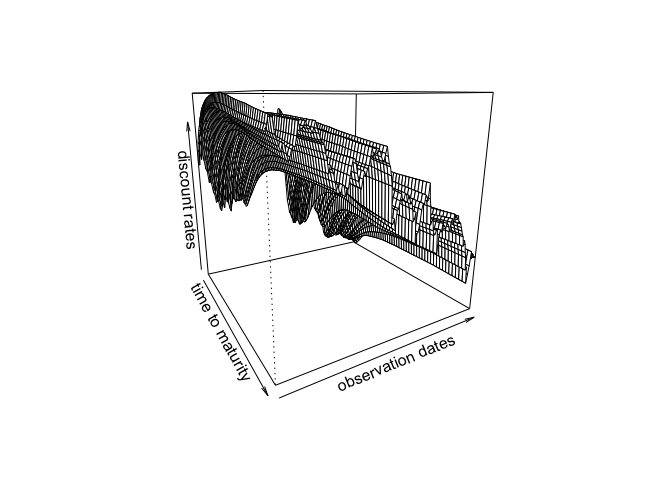
\includegraphics[width=14cm]{gfx/chapter-krls-models/bundesbank_dR.png}
\caption{Observed discount rates from Deutsche Bundesbank website, from 2002 to the end 2015}
\label{db_zerorates}
\end{figure}

\begin{table}
\begin{center}
% table caption is above the table
\caption{Summary of observed discount rates from Deutsche Bundesbank website, from 2002 to the end 2015}
\label{tab:summary_db_zeros}       % Give a unique label
% For LaTeX tables use
\begin{tabular}{llllll}
\hline\noalign{\smallskip}
Maturity & Min & 1st Qrt  & Median  & 3rd Qrt  & Max  \\
\noalign{\smallskip}\hline\noalign{\smallskip}
  1 & -0.116 & 0.858 & 2.045 & 3.072 & 5.356 \\
  5 & 0.170 & 1.327 & 2.863 & 3.807 & 5.146\\
  15 & 0.711 & 2.616 & 3.954 & 4.702 & 5.758\\
  30 & 0.805 & 2.594 & 3.962 & 4.814 & 5.784\\
  50 & 0.749 & 2.647 & 3.630 & 4.590 & 5.467\\
\noalign{\smallskip}\hline
\end{tabular}
\end{center}
\end{table}

A rolling forecasting methodology (see \cite{bergmeir2015note}) is implemented in order to obtain the benchmarks between the models. A fixed 12 months-length window for training the model, and the following 12 months for testing, the origin of the training set is then advanced of 1 month, and the training/testing procedure is repeated. The measure of forecasting performance is the Root Mean Squared Error ($RMSE$) \footnote{for a complete treatment, a validation set should be added, in order to verify that we are not 'overtraining' the models on the training set}.

\newpage

We use similar grids for all the models, in order to ease the comparability of the results, and avoid too much manual tweaking of the hyperparameters. Hence for both models, DNS-KRLS (from section \ref{sec:dnskrls}) and KRLS (from section \ref{sec:purekrls}), we consider $5$ values of $\sigma$, $l$ (the variance and length-scale parameters for Gaussian, Mat\'ern 3/2 and Mat\'ern 5/2 kernels) and $\lambda$ (the regularization parameter for all the kernels) regularly spaced between $\left[ 10^{-2}, 10^2\right]$: $10^{-2}, 10^{-1}, 1, 10, 10^{2}$. 

\medskip

For the additional parameter $\eta$ in the DNS-KRLS model, we use 5 values comprised (regularly spaced) between the minimum observed time to maturity and the maximum observed time to maturity.



\section{Conclusion}

\newpage

\nocite{wickham2016ggplot2}

